\chapter{Proposed Solution}

\section{System Overview}

The platform is implemented as a set of five independently deployable services that communicate either over HTTP or through an Apache Kafka topic. The five services are the \emph{frontend}, the \emph{primary backend}, the \emph{hook} service, the \emph{processor} service and the \emph{worker} service. A shared PostgreSQL database serves as the system of record for all persistent state, and Kafka is used as the asynchronous channel that carries action events between the processor and the worker. A high-level view of the system is shown in Figure~\ref{fig:architecture}.

\begin{figure}[h]
\centering
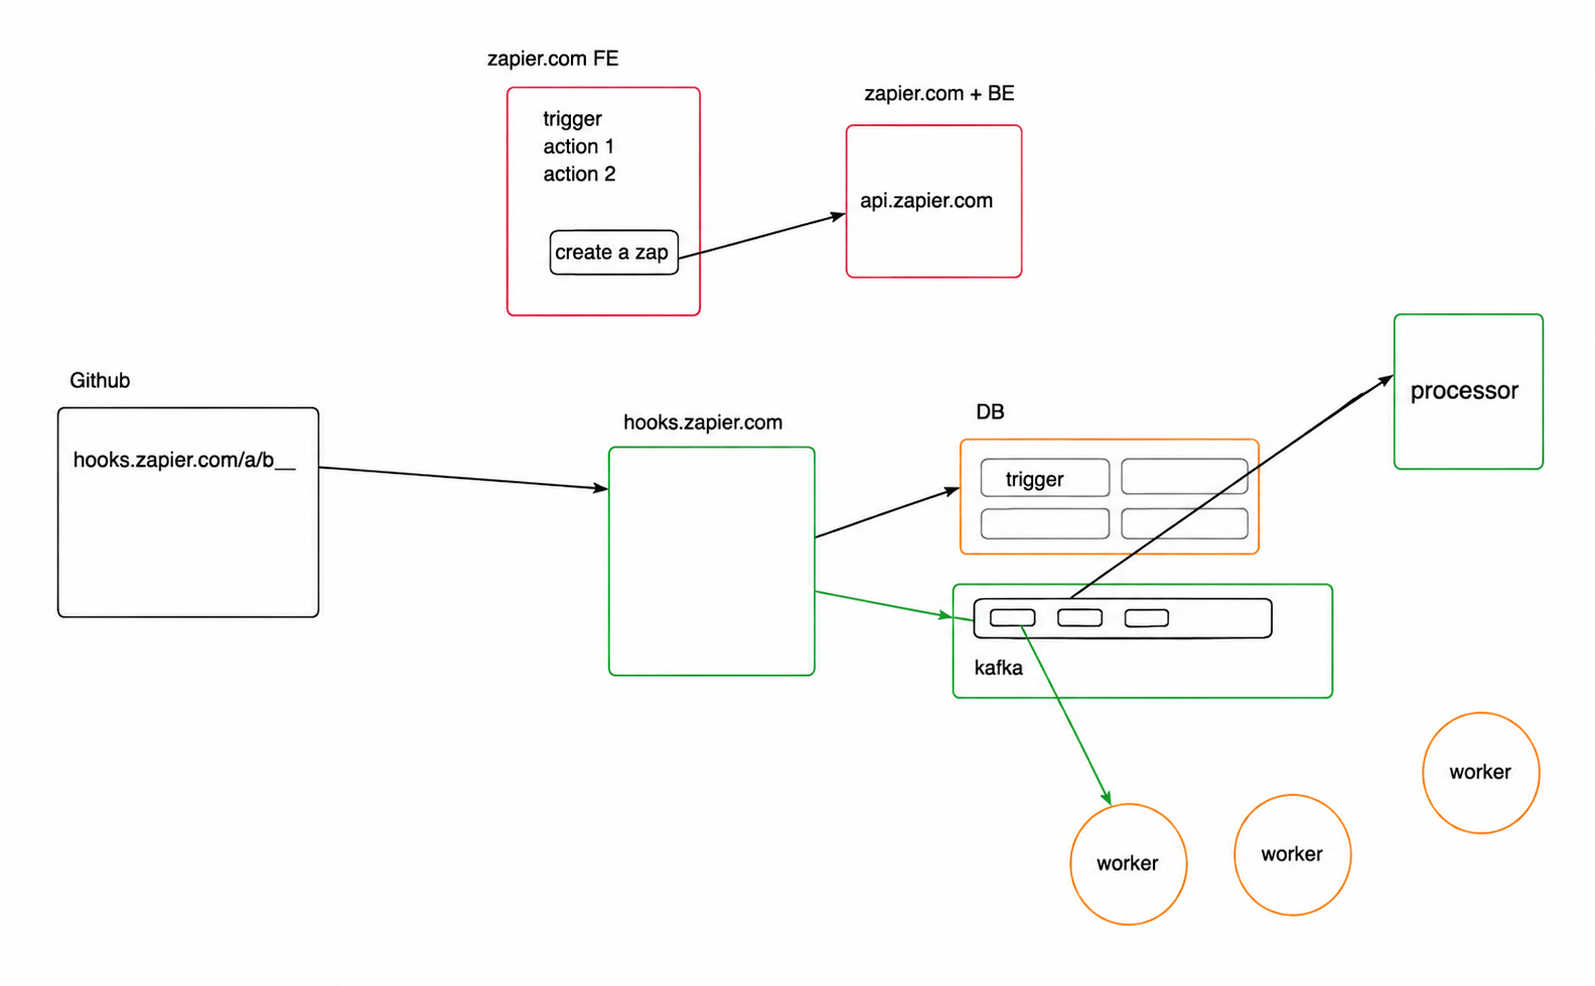
\includegraphics[width=0.95\textwidth]{figures/system-architecture.png}
\caption{High-level architecture of the platform.}
\label{fig:architecture}
\end{figure}

The diagram is organised around two complementary flows. The upper portion shows the \emph{authoring} flow: the user composes a trigger and one or more actions in the frontend (\texttt{zapier.com FE}) and submits the assembled workflow to the primary backend (\texttt{api.zapier.com}), which persists it to the database. The lower portion shows the \emph{execution} flow: an external system (illustrated in the diagram as a GitHub webhook posting to \texttt{hooks.zapier.com/a/b\_\_}) invokes the public URL served by the hook service, which records the event in the database; the processor then relays each new event from the database into Kafka; and a horizontally scalable pool of worker consumers reads from Kafka and executes the configured actions. For visual clarity the diagram omits the read-only database accesses performed by the primary backend when serving API requests and by the worker when loading the Zap definition before each action; both are described in the corresponding service sections later in this chapter.

The end-to-end lifecycle of a single workflow execution proceeds as follows. A user first authenticates against the primary backend through the frontend, creates a workflow, and receives a unique public webhook URL bound to that workflow. When that URL is later invoked by an external system, the hook service accepts the request and persists a \texttt{ZapRun} row together with a \texttt{ZapRunOutbox} row in a single database transaction. The processor service continuously polls the outbox table and, for each entry it finds, produces a corresponding message to the \texttt{zap-events} Kafka topic before deleting the outbox row. The worker service consumes messages from that topic; for each message it loads the relevant workflow definition, executes the appropriate action (e.g.\ email or Solana transfer), and if the workflow has further actions remaining, republishes the same message with an incremented stage number so that the next action can be processed by the same consumer group. Figure~\ref{fig:webhook-sequence} traces the corresponding sequence of messages between the services for a single Zap run.

\begin{figure}[h]
\centering
\begin{tikzpicture}[
    actor/.style={draw, thick, rounded corners=2pt, minimum width=1.7cm, minimum height=0.7cm, align=center, font=\small\bfseries, fill=gray!12},
    lifeline/.style={dashed, gray!70, thick},
    msg/.style={->, thick, >=Stealth, font=\scriptsize},
    msgret/.style={->, thick, dashed, >=Stealth, gray!55!black, font=\scriptsize},
    phase/.style={draw=gray!60, thick, rounded corners=2pt, minimum height=0.5cm, font=\scriptsize\itshape, align=left, fill=yellow!12, inner sep=3pt}
]
\def\xExt{0}
\def\xHook{2.2}
\def\xDb{4.4}
\def\xProc{6.6}
\def\xKafka{8.8}
\def\xWorker{11.0}

% Actor headers
\node[actor] (ext)    at (\xExt,    0) {External\\System};
\node[actor] (hook)   at (\xHook,   0) {Hook};
\node[actor] (db)     at (\xDb,     0) {DB};
\node[actor] (proc)   at (\xProc,   0) {Processor};
\node[actor] (kafka)  at (\xKafka,  0) {Kafka};
\node[actor] (worker) at (\xWorker, 0) {Worker};

% Lifelines
\foreach \x in {\xExt, \xHook, \xDb, \xProc, \xKafka, \xWorker} {
    \draw[lifeline] (\x, -0.4) -- (\x, -12.3);
}

% --- Phase 1: Webhook ingestion ---
\node[phase, anchor=west, minimum width=12cm] at (-0.85, -0.95) {1. Webhook ingestion via transactional outbox};

\draw[msg]    (\xExt,  -1.55) -- node[above] {POST \texttt{/hooks/catch/...}} (\xHook, -1.55);
\draw[msg]    (\xHook, -2.20) -- node[above] {INSERT ZapRun + ZapRunOutbox (single txn)} (\xDb, -2.20);
\draw[msgret] (\xHook, -2.90) -- node[above] {HTTP 200} (\xExt, -2.90);

% --- Phase 2: Processor relay ---
\node[phase, anchor=west, minimum width=12cm] at (-0.85, -3.50) {2. Processor relay loop (poll $\sim$2\,s)};

\draw[msg]    (\xProc, -4.10) -- node[above] {SELECT outbox rows} (\xDb, -4.10);
\draw[msgret] (\xDb,   -4.65) -- node[above] {rows[\,]} (\xProc, -4.65);
\draw[msg]    (\xProc, -5.25) -- node[above] {produce \{zapRunId, stage:\,0\}} (\xKafka, -5.25);
\draw[msg]    (\xProc, -5.90) -- node[above] {DELETE outbox row} (\xDb, -5.90);

% --- Phase 3: Worker execution ---
\node[phase, anchor=west, minimum width=12cm] at (-0.85, -6.50) {3. Worker executes one action per consumed message};

\draw[msg]    (\xKafka,  -7.10) -- node[above] {consume \{stage:\,N\}} (\xWorker, -7.10);
\draw[msg]    (\xWorker, -7.85) -- node[above] {SELECT Zap with actions} (\xDb, -7.85);
\draw[msgret] (\xDb,     -8.45) -- node[above] {zap, actions[\,]} (\xWorker, -8.45);

% Self-message on Worker: outbound call to external action service
\draw[msg, ->, thick] (\xWorker + 0.1, -9.10) to[out=0, in=0, looseness=4] (\xWorker + 0.1, -9.70);
\node[font=\scriptsize, anchor=west, align=left] at (\xWorker + 0.65, -9.40) {execute action\\(SMTP / Solana RPC)};

\draw[msg] (\xWorker, -10.50) -- node[above] {if more actions: produce \{stage:\,N+1\}} (\xKafka, -10.50);
\draw[msg] (\xWorker, -11.25) -- node[above] {commit offset} (\xKafka, -11.25);

% Closing note
\node[phase, anchor=west, minimum width=12cm, fill=yellow!8] at (-0.85, -11.90) {stages repeat on the same lifelines until the last action, after which no follow-up is produced};

\end{tikzpicture}
\caption{End-to-end sequence of messages for a single Zap run, from external webhook reception through action execution. Solid arrows denote synchronous calls; dashed arrows denote return values. The self-arrow on the \emph{Worker} lifeline represents the outbound call to the external service that the chosen action targets (SMTP relay for the \texttt{email} action or Solana RPC for the \texttt{send-sol} action).}
\label{fig:webhook-sequence}
\end{figure}

This division of responsibilities directly addresses the functional and non-functional requirements stated in Chapter~3. Durability of accepted events is provided by the transactional outbox table; ordered, at-least-once execution of actions is provided by the combination of the \texttt{sortingOrder} field and Kafka's manual offset commits; horizontal scalability of the worker is provided by Kafka's consumer-group abstraction; and the operability requirement is met by packaging every service as a Docker container that is brought up from a single Compose file.

\section{Database Design}

All persistent state is stored in a single PostgreSQL database whose schema is managed by Prisma migrations. The schema comprises seven tables, summarised in Table~\ref{tab:schema}.

\begin{table}[h]
\centering
\caption{Core tables of the database schema.}
\label{tab:schema}
\renewcommand{\arraystretch}{1.3}
\begin{tabular}{|p{3.2cm}|p{10cm}|}
\hline
\textbf{Table} & \textbf{Purpose} \\ \hline
\texttt{User} & Stores registered users. Fields: \texttt{id}, \texttt{name}, \texttt{email}, \texttt{password} (bcrypt-hashed). \\ \hline
\texttt{Zap} & Represents a single workflow owned by a user. Holds references to the associated trigger and actions. \\ \hline
\texttt{AvailableTrigger} & Catalogue of trigger types known to the platform (currently only ``webhook''). \\ \hline
\texttt{Trigger} & Concrete trigger instance attached to a single Zap, with a JSON \texttt{metadata} column for configuration. \\ \hline
\texttt{AvailableAction} & Catalogue of action types known to the platform (email, send-sol). \\ \hline
\texttt{Action} & Concrete action instance attached to a Zap, with \texttt{metadata} and a \texttt{sortingOrder} that defines execution position. \\ \hline
\texttt{ZapRun} & One row per execution of a Zap, carrying the webhook payload in a JSON \texttt{metadata} column. \\ \hline
\texttt{ZapRunOutbox} & Transactional outbox row associated with a single \texttt{ZapRun}. Inserted in the same transaction as the \texttt{ZapRun} and later deleted by the processor. \\ \hline
\end{tabular}
\end{table}

The use of a JSON column for trigger and action metadata is a deliberate design choice: it allows new trigger and action types to be added to the catalogue without any schema migration, since each type is free to define the shape of its own metadata. Only the skeleton of the relational model, with its foreign-key constraints, is enforced at the database level. The separation between \texttt{AvailableAction} (the type) and \texttt{Action} (the instance) is analogous to the separation between a class and its instances in an object-oriented language. The full entity-relationship diagram for the schema, generated from the live Prisma model, is shown in Figure~\ref{fig:schema-er}.

\begin{figure}[h]
\centering
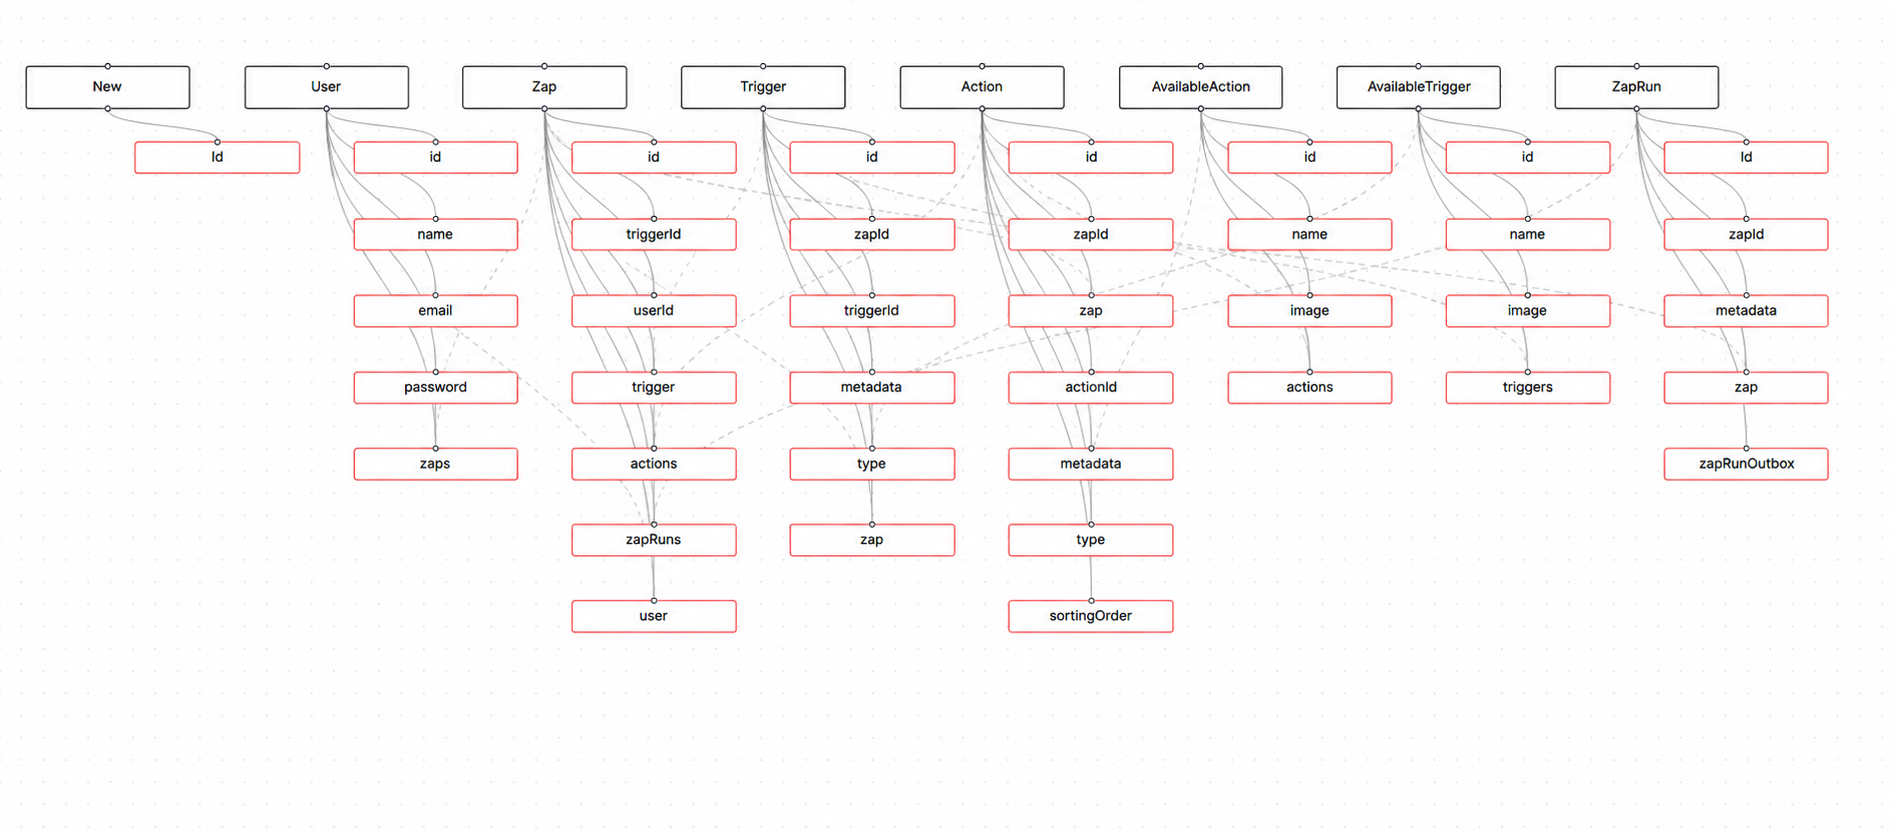
\includegraphics[width=\textwidth]{figures/database-schema.png}
\caption{Entity-relationship diagram of the database schema.}
\label{fig:schema-er}
\end{figure}

\section{Primary Backend Service}

The primary backend is an Express application written in TypeScript. It is the only service that frontend clients communicate with, and it is responsible for authentication and for all create / read operations on user-owned resources. All input is validated against Zod schemas before any business logic executes, and the resulting typed objects are passed to Prisma for persistence. Authentication is handled by a middleware function that extracts a JSON Web Token from the \texttt{Authorization} header, verifies it against a secret, and attaches the decoded user identifier to the request object for downstream handlers. Figure~\ref{fig:login-network} shows the browser developer-tools view of a sign-in request being issued against the local backend, with the underlying \texttt{POST /api/v1/user/signin} call visible in the Network panel. The REST endpoints exposed by the service are summarised in Table~\ref{tab:endpoints}.

\begin{figure}[h]
\centering
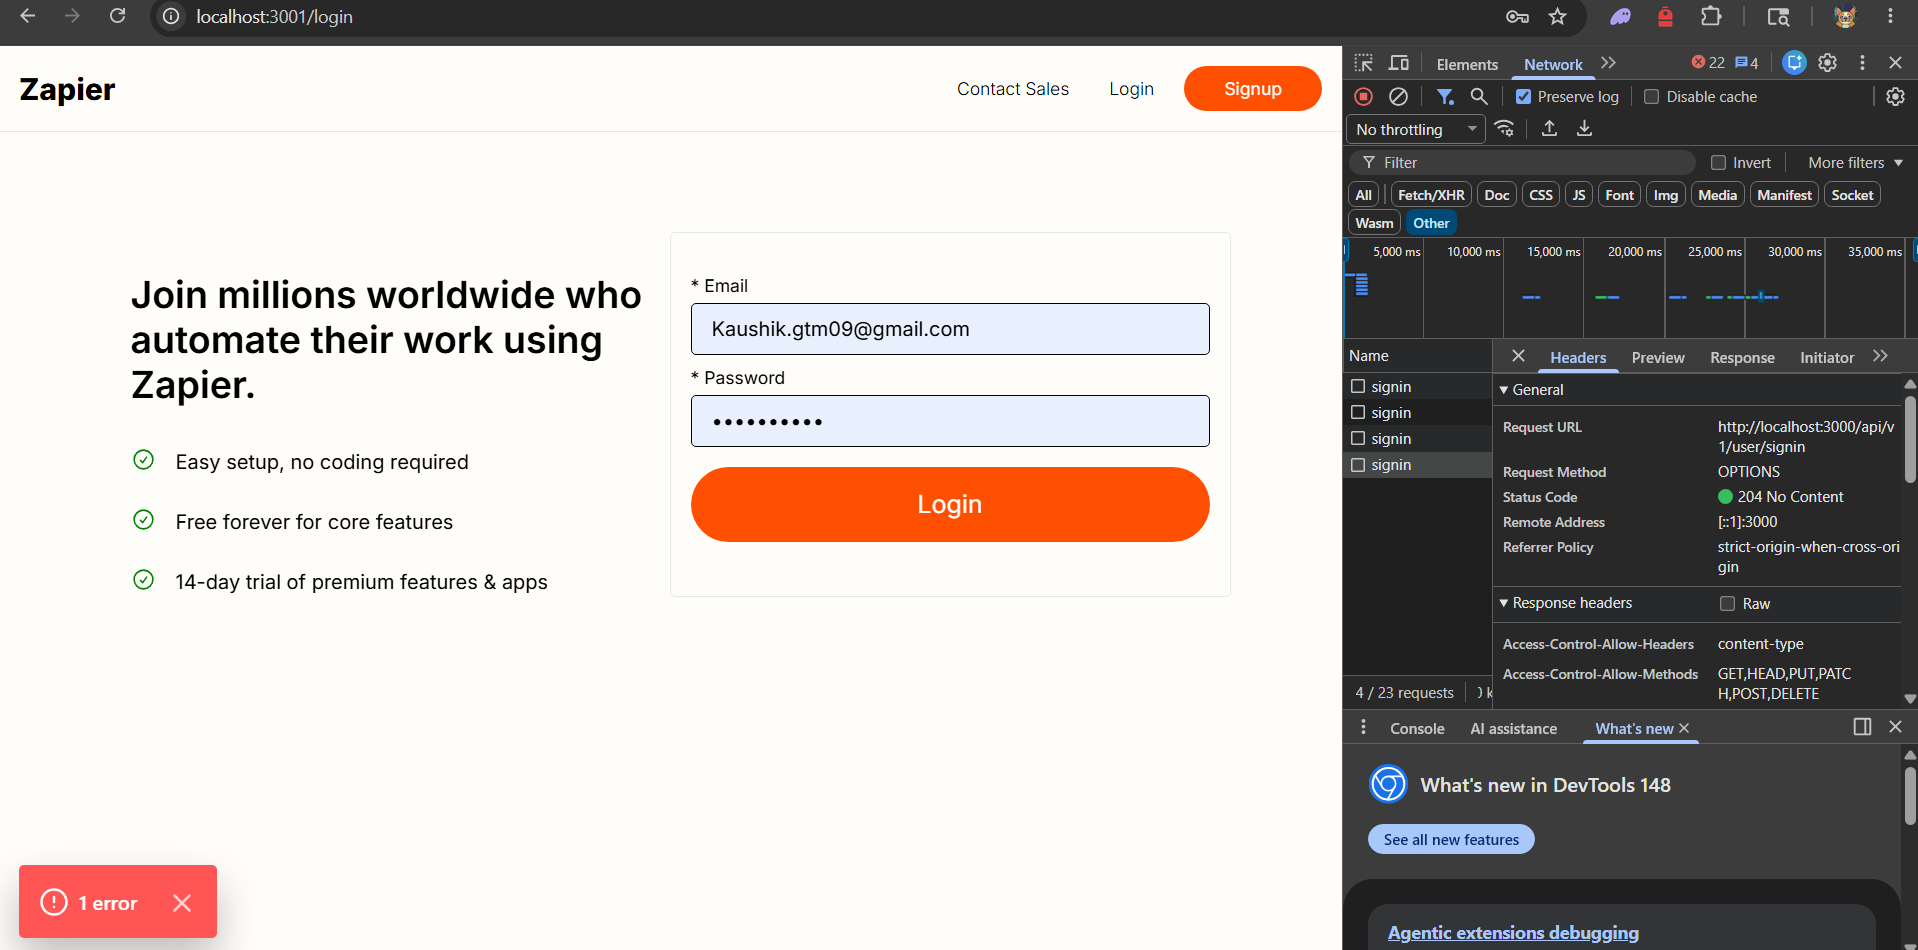
\includegraphics[width=0.95\textwidth]{figures/ui-login-network.png}
\caption{Sign-in request as observed in the browser developer tools. The login form on the left invokes \texttt{POST /api/v1/user/signin} against the primary backend; the request and response are visible in the Network panel on the right, demonstrating that the authentication endpoint is reachable and returning a token.}
\label{fig:login-network}
\end{figure}

\begin{table}[h]
\centering
\caption{REST endpoints exposed by the primary backend.}
\label{tab:endpoints}
\renewcommand{\arraystretch}{1.3}
\begin{tabular}{|l|p{4.2cm}|c|p{5.0cm}|}
\hline
\textbf{Method} & \textbf{Path} & \textbf{Auth} & \textbf{Purpose} \\ \hline
POST & \texttt{/api/v1/user/signup} & No & Register a new user. \\ \hline
POST & \texttt{/api/v1/user/signin} & No & Authenticate and issue a JWT. \\ \hline
GET & \texttt{/api/v1/user} & Yes & Fetch the authenticated user's profile. \\ \hline
POST & \texttt{/api/v1/zap} & Yes & Create a new Zap with trigger and actions. \\ \hline
GET & \texttt{/api/v1/zap} & Yes & List all Zaps owned by the user. \\ \hline
GET & \texttt{/api/v1/zap/:zapId} & Yes & Fetch a single Zap including its actions. \\ \hline
GET & \texttt{/api/v1/trigger/available} & No & List all available trigger types. \\ \hline
GET & \texttt{/api/v1/action/available} & No & List all available action types. \\ \hline
\end{tabular}
\end{table}

The \texttt{POST /api/v1/zap} handler is worth describing in detail because it coordinates multiple table inserts. It begins a single Prisma transaction in which it first creates the \texttt{Zap} row with an empty \texttt{triggerId}, then creates all of the requested \texttt{Action} rows with appropriate \texttt{sortingOrder} values, then creates the \texttt{Trigger} row that references the \texttt{Zap}, and finally updates the \texttt{Zap.triggerId} field to point at the newly created trigger. Because all four operations are executed inside a single transaction, the database is never observed in a partially constructed state.

\section{Hook Service}

The hook service is a minimal Express application whose sole responsibility is to receive webhook requests from external systems and enqueue them for asynchronous processing. It exposes a single endpoint, \texttt{POST /hooks/catch/:userId/:zapId}, which accepts an arbitrary JSON body and returns a short acknowledgement. For every request received, it executes a single Prisma transaction that inserts one row into \texttt{ZapRun} (carrying the incoming payload in the \texttt{metadata} column) and one row into \texttt{ZapRunOutbox} (referencing the \texttt{ZapRun}). A simplified version of the relevant code is shown in Listing~\ref{lst:hook}.

\begin{lstlisting}[language=JavaScript, caption={Transactional outbox insert in the hook service.}, label=lst:hook]
app.post("/hooks/catch/:userId/:zapId", async (req, res) => {
    const { userId, zapId } = req.params;
    const body = req.body;
    await client.$transaction(async (tx) => {
        const run = await tx.zapRun.create({
            data: { zapId, metadata: body }
        });
        await tx.zapRunOutbox.create({
            data: { zapRunId: run.id }
        });
    });
    res.json({ message: "webhook received" });
});
\end{lstlisting}

The design consequence of this pattern is that, from the moment the transaction commits, the platform has accepted responsibility for eventually executing the associated actions. Neither the processor nor the Kafka cluster needs to be reachable at the instant the webhook arrives. Should the processor be down, the \texttt{ZapRunOutbox} rows simply accumulate in the database; when the processor resumes, it drains the backlog and the platform catches up.

\section{Processor Service}

The processor is a headless Node.js service that continuously polls the \texttt{ZapRunOutbox} table, relays the contents to Kafka and deletes the processed rows. Its control loop is intentionally simple: on each iteration it fetches up to ten outbox rows; if none are found, it sleeps for two seconds and tries again; if rows are found, it produces a message for each row to the \texttt{zap-events} Kafka topic and then performs a \texttt{deleteMany} on the rows it just sent. Messages have the JSON shape \texttt{\{"zapRunId": <uuid>, "stage": 0\}}, where the \texttt{stage} field indicates which position in the action chain should be executed next.

Because the polling query and the delete are not wrapped in a transaction with the producer's \texttt{send} call, in principle a crash between the send and the delete could cause an outbox row to be published twice. The platform accepts this \emph{at-least-once} delivery semantic deliberately: the worker is idempotent in practice because it identifies its work by \texttt{zapRunId} and \texttt{stage}, and duplicate executions of an action (e.g.\ sending the same email twice) are considered acceptable given the target use-case. An at-most-once alternative would require a two-phase commit that is not justified by the present requirements.

\section{Worker Service}

The worker is a Kafka consumer that performs the actual execution of actions. It joins the consumer group \texttt{main-worker-2} and subscribes to the \texttt{zap-events} topic. Automatic offset commits are disabled; the worker only commits offsets after the action has been successfully executed, so that in the event of a crash the failed message is re-delivered on restart. The worker currently supports two action types, described in Table~\ref{tab:actions}.

\begin{table}[h]
\centering
\caption{Action types supported by the worker.}
\label{tab:actions}
\renewcommand{\arraystretch}{1.3}
\begin{tabular}{|l|p{4.5cm}|p{7cm}|}
\hline
\textbf{Action ID} & \textbf{Metadata fields} & \textbf{Behaviour} \\ \hline
\texttt{email} & \texttt{email}, \texttt{body} & Sends a transactional email over SMTP using Nodemailer to the recipient address after placeholder substitution against the webhook payload. \\ \hline
\texttt{send-sol} & \texttt{address}, \texttt{amount} & Constructs and signs a Solana transfer transaction using the \texttt{@solana/web3.js} library, then submits it to the Solana mainnet RPC endpoint. \\ \hline
\end{tabular}
\end{table}

For every consumed message the worker loads the corresponding \texttt{Zap} together with its actions from the database, selects the action whose \texttt{sortingOrder} equals the message's \texttt{stage}, and executes it. Before execution, the action's metadata (which may contain placeholders such as \texttt{\{payment.amount\}}) is passed through a simple template parser that substitutes values taken from the webhook payload stored on the \texttt{ZapRun}. If the current stage is not the last action of the Zap, the worker produces a follow-up message to the same Kafka topic with an incremented stage, thereby driving the next step of the workflow. If the current stage is the last, no follow-up is produced and the offset is committed. Figure~\ref{fig:worker-stages} illustrates this self-republishing loop for a three-action Zap.

\begin{figure}[h]
\centering
\begin{tikzpicture}[
    msg/.style={draw, thick, rounded corners=2pt, minimum width=2.4cm, minimum height=1.0cm, align=center, font=\small, fill=blue!5},
    worker/.style={draw, thick, rounded corners=2pt, minimum width=2.8cm, minimum height=1.4cm, align=center, font=\small, fill=orange!10},
    lanelabel/.style={font=\bfseries\small, align=right, anchor=east},
    >={Stealth[length=2mm]}
]
% Lane labels
\node[lanelabel] at (-1.8, 2.1) {Kafka topic};
\node[lanelabel] at (-1.8, -1.9) {Worker};

% Messages on the topic
\node[msg] (m0) at (0, 2.1) {\{zapRunId,\\ stage:\,0\}};
\node[msg] (m1) at (4, 2.1) {\{zapRunId,\\ stage:\,1\}};
\node[msg] (m2) at (8, 2.1) {\{zapRunId,\\ stage:\,2\}};

% Worker iterations
\node[worker] (w0) at (0, -1.9) {execute action at\\ \texttt{sortingOrder}\,=\,0\\ (e.g.\ \texttt{email})};
\node[worker] (w1) at (4, -1.9) {execute action at\\ \texttt{sortingOrder}\,=\,1\\ (e.g.\ \texttt{send-sol})};
\node[worker] (w2) at (8, -1.9) {last action;\\ commit offset,\\ no follow-up};

% Consume arrows (Kafka -> Worker)
\draw[->, thick] (m0) -- node[right, font=\scriptsize] {consume} (w0);
\draw[->, thick] (m1) -- node[right, font=\scriptsize] {consume} (w1);
\draw[->, thick] (m2) -- node[right, font=\scriptsize] {consume} (w2);

% Produce arrows (Worker -> Kafka, with stage+1)
\draw[->, thick, blue!55!black, dashed]
  (w0.north east) .. controls +(1.0,1.4) and +(-1.0,-1.4) ..
  node[midway, sloped, above, font=\scriptsize] {produce \{stage:\,1\}} (m1.south west);
\draw[->, thick, blue!55!black, dashed]
  (w1.north east) .. controls +(1.0,1.4) and +(-1.0,-1.4) ..
  node[midway, sloped, above, font=\scriptsize] {produce \{stage:\,2\}} (m2.south west);
\end{tikzpicture}
\caption{Sequential execution of a three-action Zap through worker self-republishing. Each consumed message at \texttt{stage}\,$=N$ causes the worker to execute the action whose \texttt{sortingOrder}\,$=N$; if further actions remain the worker produces a follow-up message with \texttt{stage}\,$=N{+}1$ to the same Kafka topic. On the final action no follow-up is produced and the consumer-group offset is committed.}
\label{fig:worker-stages}
\end{figure}

This design keeps the worker entirely stateless between messages. All progress is tracked by the combination of the Kafka offset and the \texttt{stage} field inside the message. A worker crash therefore cannot cause an action to be skipped: either the offset was committed (and the action was executed) or it was not (and the message will be re-delivered).

\section{Frontend and Deployment}

The frontend is a Next.js application written in TypeScript and styled with Tailwind CSS. It consists of four principal pages: a landing page, a sign-up form, a sign-in form, and a dashboard, illustrated in Figures~\ref{fig:ui-public} and~\ref{fig:ui-auth}. From the dashboard the user can list existing Zaps, copy their unique public webhook URL, and navigate to a Zap-builder screen. The Zap builder, shown in Figure~\ref{fig:ui-zap-builder}, fetches the catalogues of available triggers and actions from the primary backend, and lets the user assemble a workflow visually by clicking a trigger and then appending actions one at a time. Each action presents a small form whose fields are determined by the action type; the form values become the JSON \texttt{metadata} stored on the \texttt{Action} row. Submitting the builder issues a single \texttt{POST /api/v1/zap} call to the backend.

\begin{figure}[h]
\centering
\begin{minipage}[t]{0.48\textwidth}
    \centering
    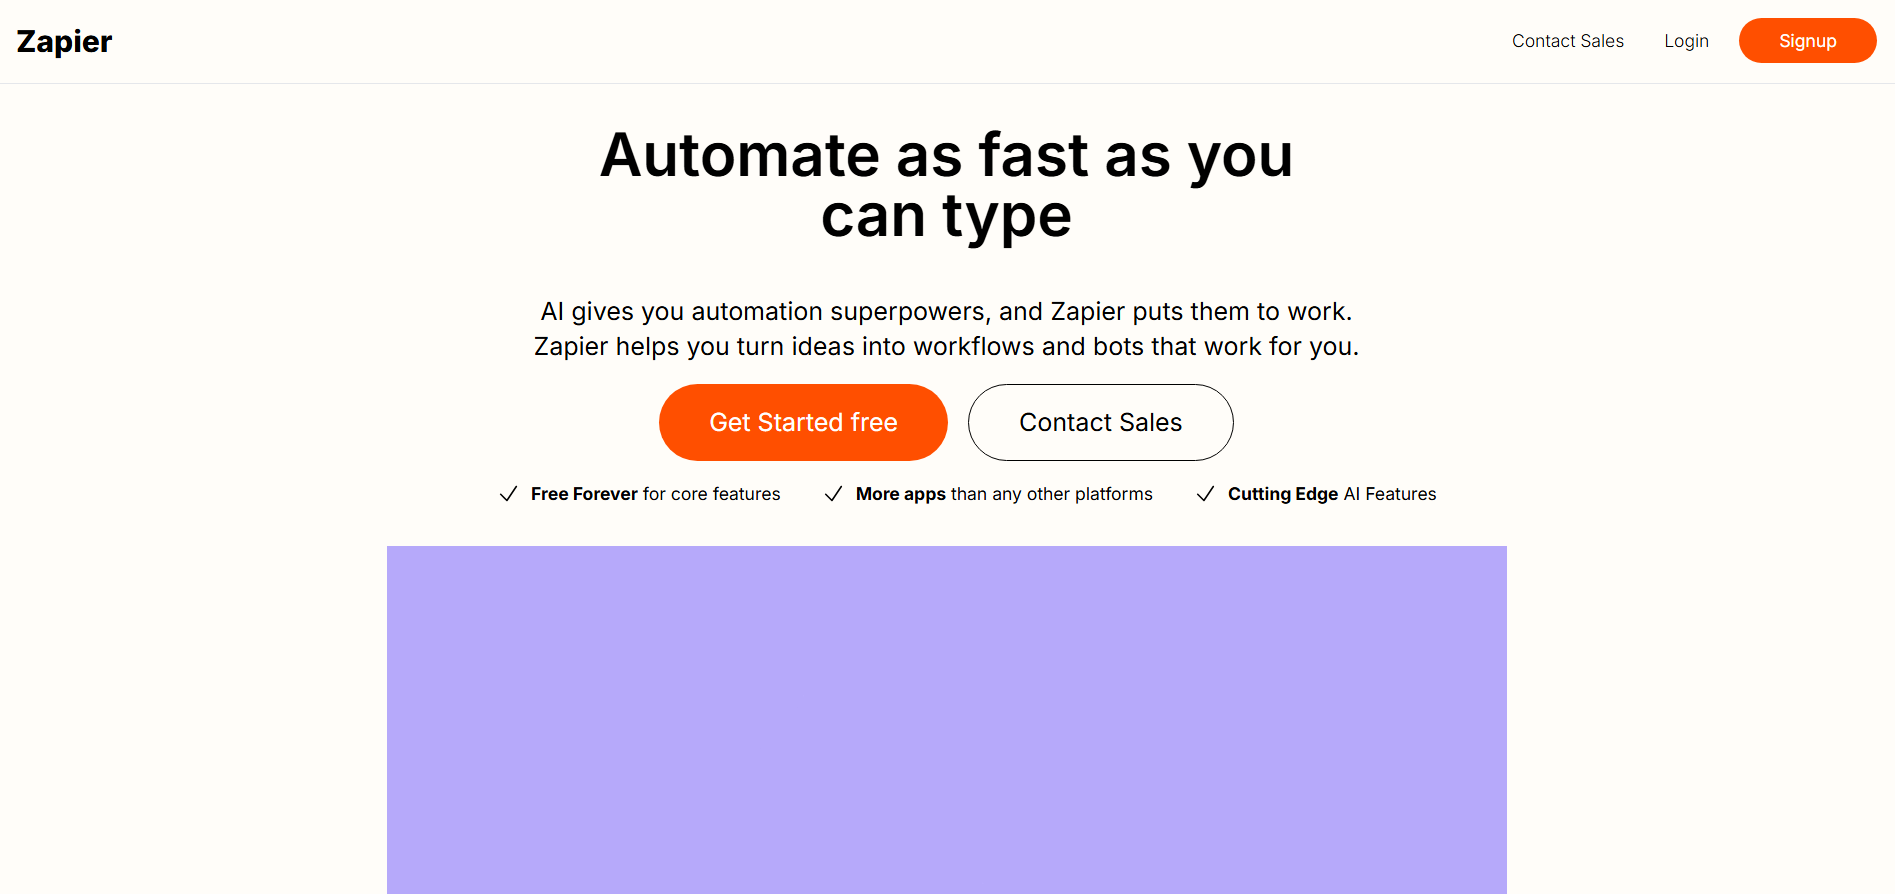
\includegraphics[width=\linewidth]{figures/ui-landing.png}\\[2pt]
    {\small\textbf{(a)} Landing page}
\end{minipage}\hfill
\begin{minipage}[t]{0.48\textwidth}
    \centering
    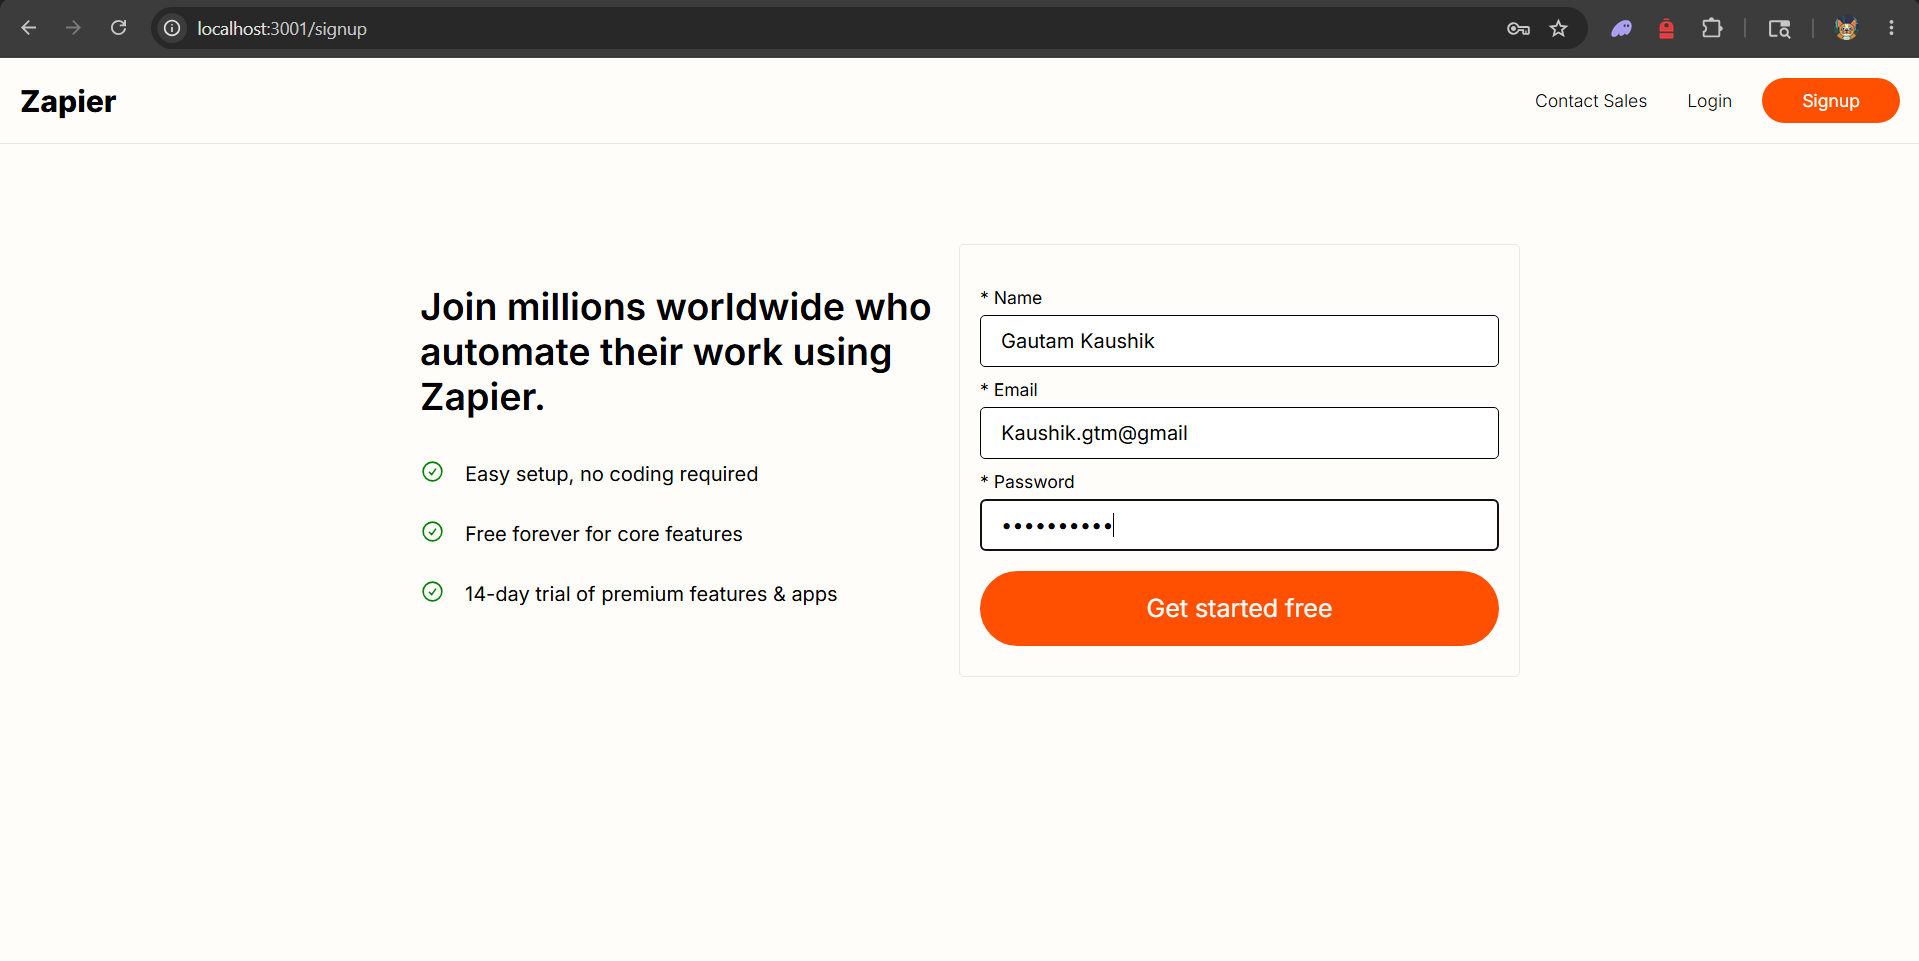
\includegraphics[width=\linewidth]{figures/ui-signup.png}\\[2pt]
    {\small\textbf{(b)} Signup form}
\end{minipage}
\caption{Public-facing frontend pages. The landing page (a) is the unauthenticated entry point; the signup form (b) posts to \texttt{POST /api/v1/user/signup}, after which the user is redirected to the dashboard.}
\label{fig:ui-public}
\end{figure}

\begin{figure}[h]
\centering
\begin{minipage}[t]{0.48\textwidth}
    \centering
    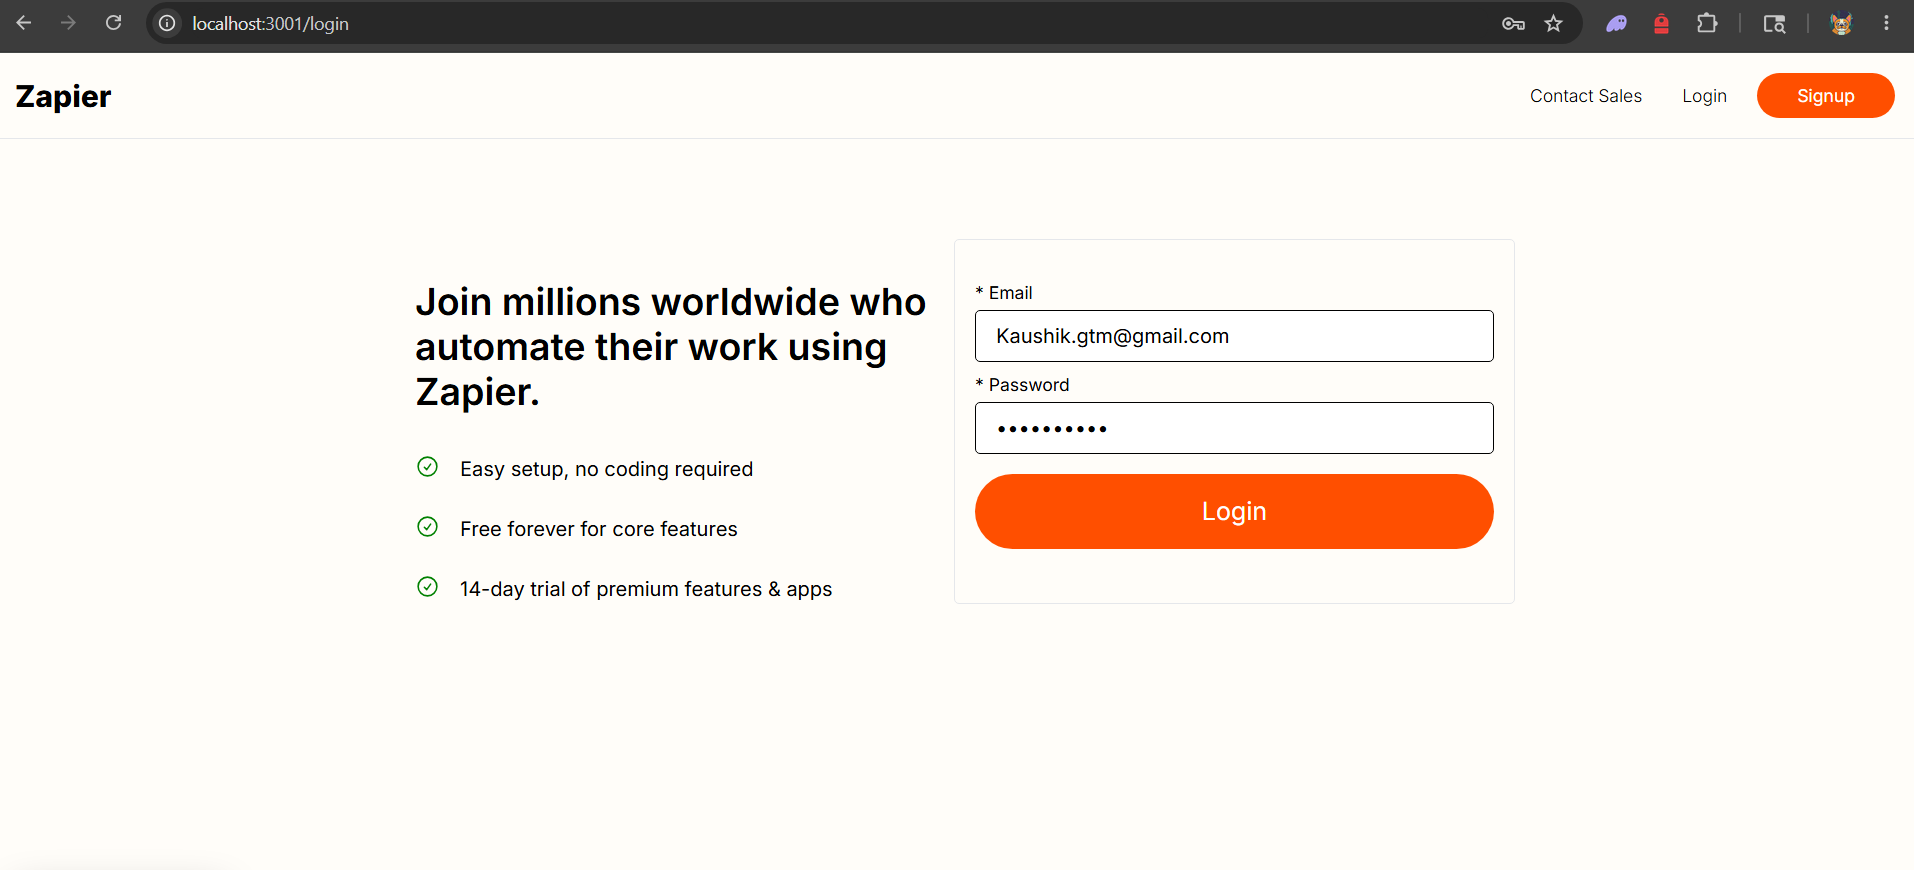
\includegraphics[width=\linewidth]{figures/ui-login.png}\\[2pt]
    {\small\textbf{(a)} Sign-in form}
\end{minipage}\hfill
\begin{minipage}[t]{0.48\textwidth}
    \centering
    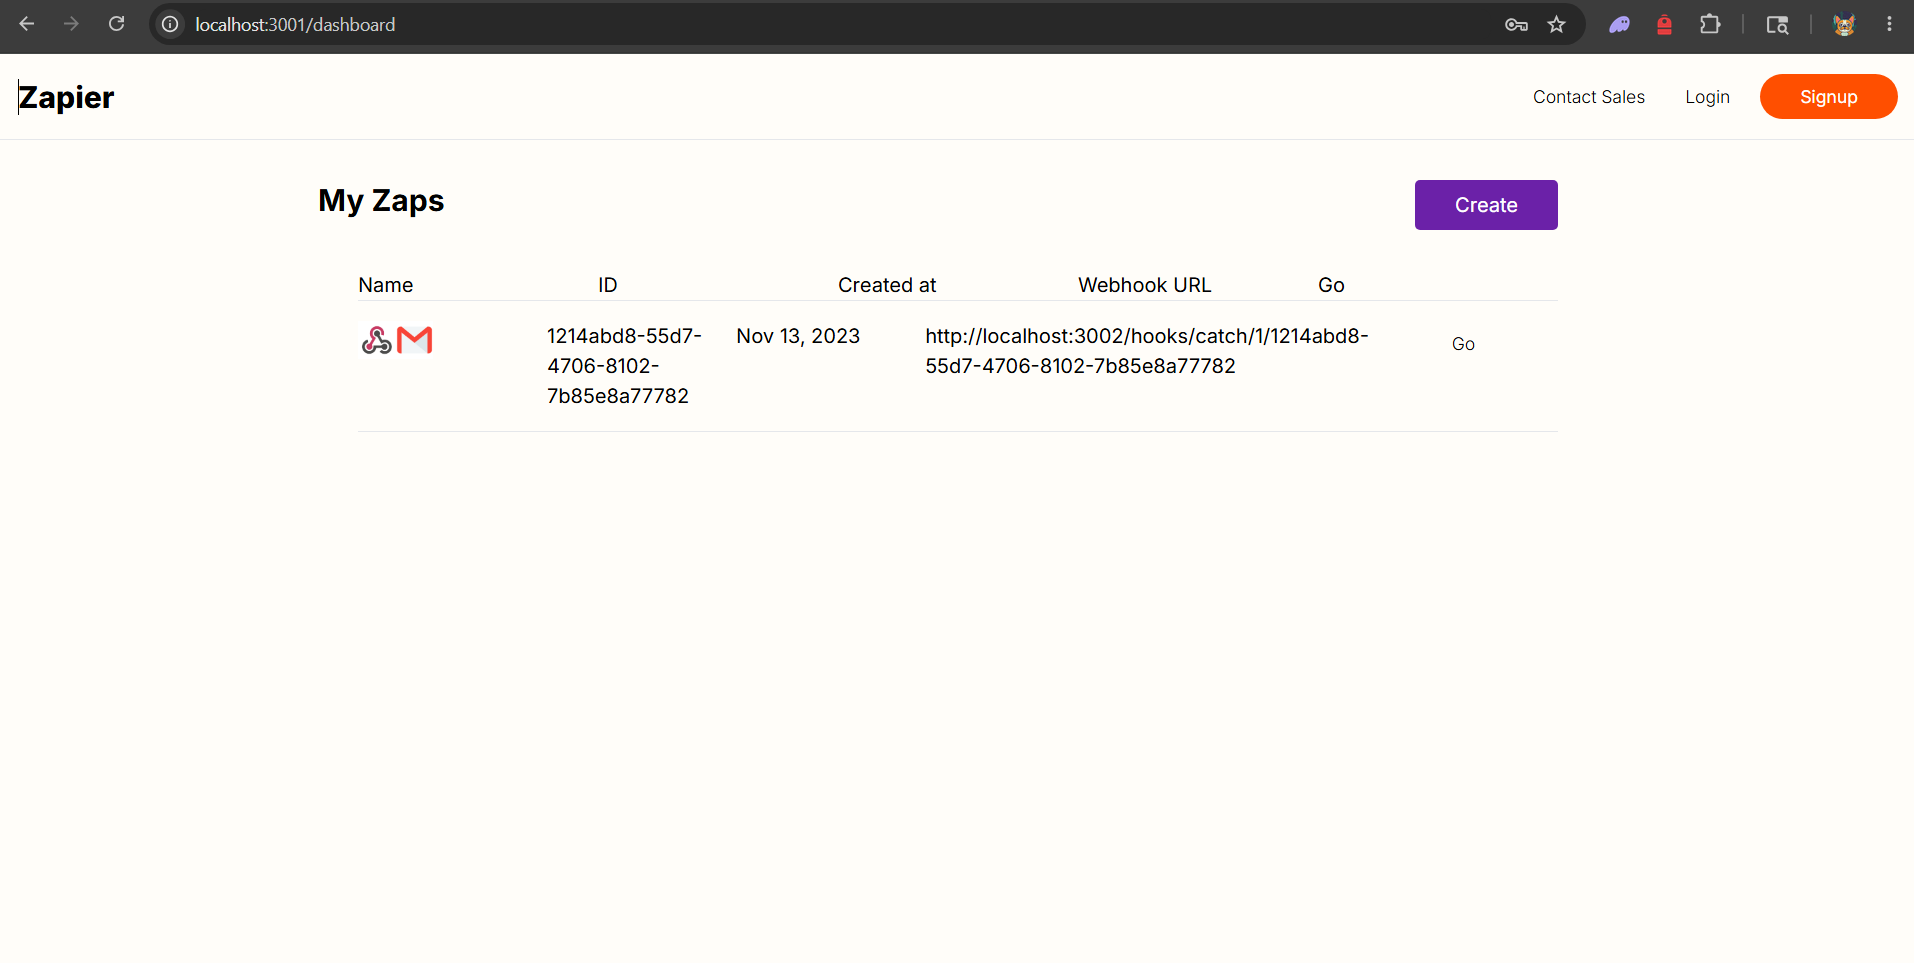
\includegraphics[width=\linewidth]{figures/ui-dashboard.png}\\[2pt]
    {\small\textbf{(b)} Dashboard listing the user's Zaps}
\end{minipage}
\caption{Authenticated user surfaces. Submitting the sign-in form (a) issues a JWT that is attached to all subsequent API calls; the dashboard (b) lists each Zap together with its unique public webhook URL that external systems can POST to in order to fire the workflow.}
\label{fig:ui-auth}
\end{figure}

\begin{figure}[h]
\centering
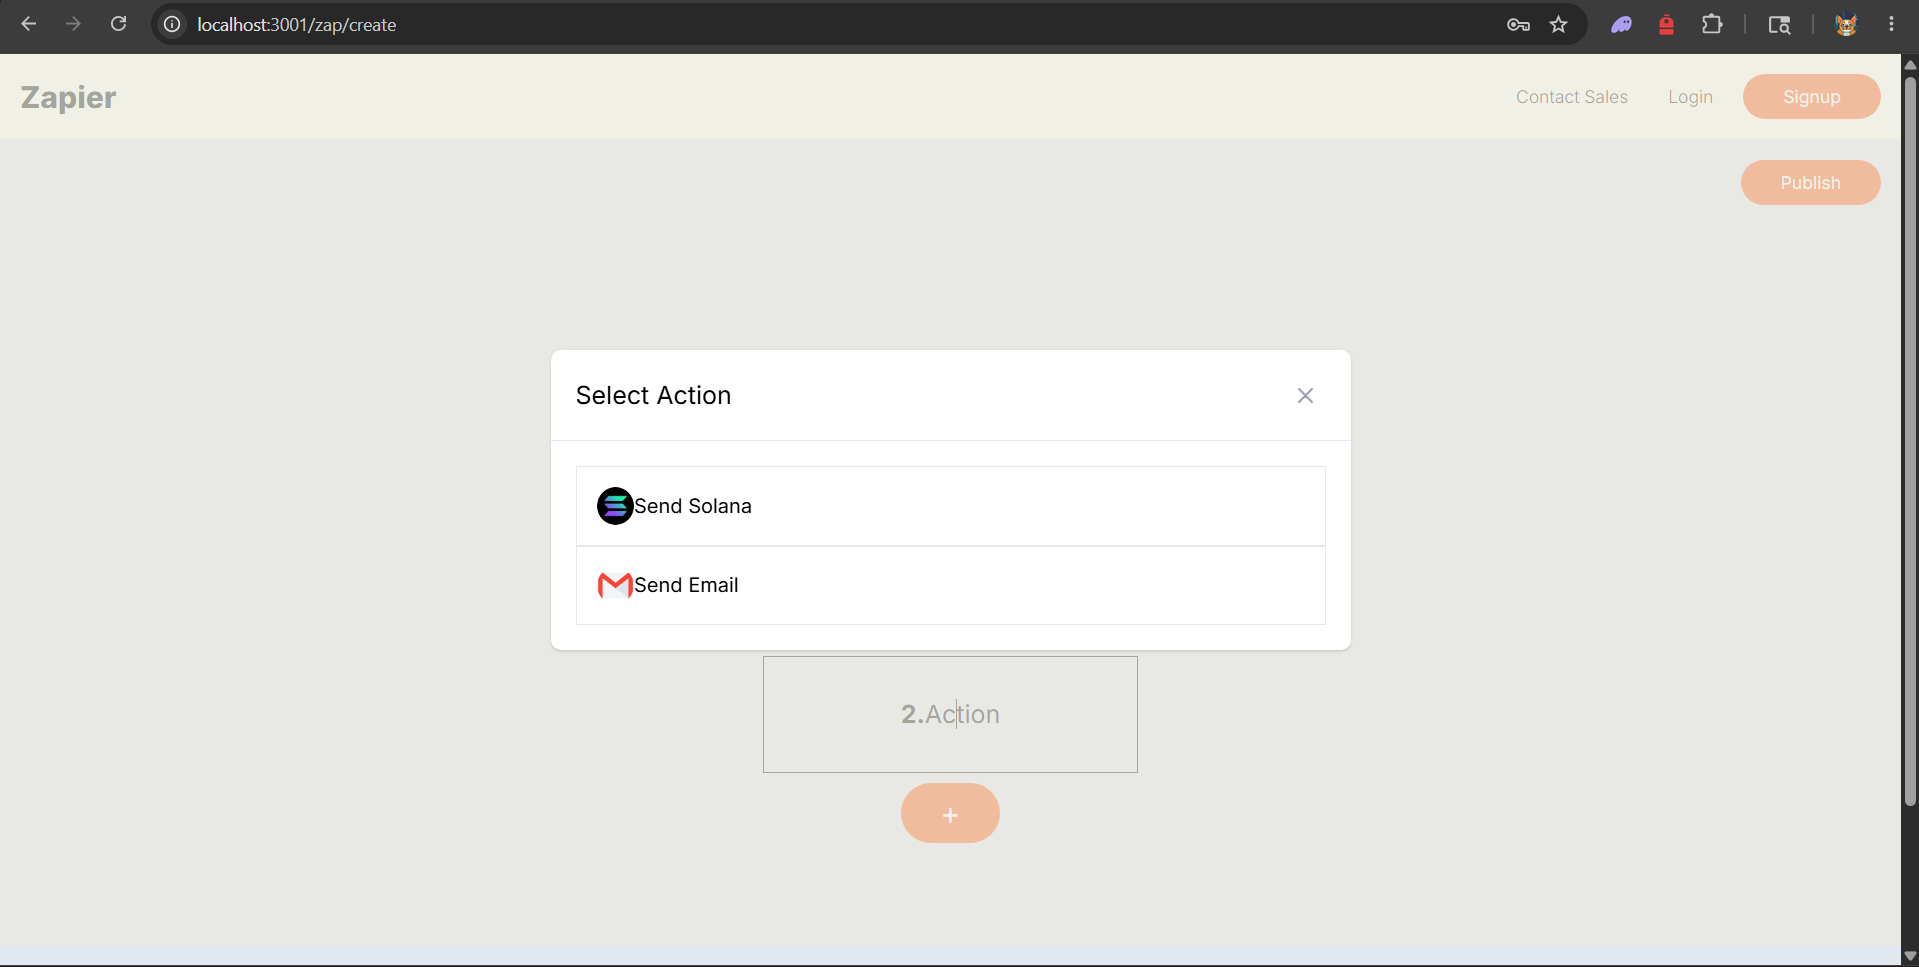
\includegraphics[width=0.9\textwidth]{figures/ui-zap-builder.png}
\caption{The Zap-builder screen with the action-selection modal open. Available actions are fetched dynamically from \texttt{GET /api/v1/action/available}, so adding a new server-side action type makes it immediately selectable in the UI without any frontend change.}
\label{fig:ui-zap-builder}
\end{figure}

Every service is containerised using a dedicated \texttt{Dockerfile} and can be brought up locally using the provided \texttt{docker-compose.yml}, which additionally launches a single-broker Kafka cluster (with Zookeeper) on port 9092. A second compose file, \texttt{docker-compose.prod.yml}, references pre-built images from Docker Hub and is intended for production deployment on a single virtual machine. Figure~\ref{fig:cicd} shows the structure of the CI/CD pipeline, which is implemented as a GitHub Actions workflow. On each push to \texttt{main}, the pipeline first detects which service directories have changed, then builds and pushes a new Docker image to Docker Hub for each changed service, and finally connects to the deployment host over SSH and restarts only the containers whose images were rebuilt. This strategy keeps deployments fast and minimises downtime.

\begin{figure}[h]
\centering
\begin{tikzpicture}[
    node distance=0.7cm,
    box/.style={draw, thick, minimum width=3.5cm, minimum height=0.9cm, align=center, rounded corners=2pt, font=\small},
    >={Stealth[length=2mm]}
]
\node[box] (push) {Push to main};
\node[box, below=of push] (detect) {Detect changed services};
\node[box, below=of detect] (build) {Build \& push Docker images};
\node[box, below=of build] (deploy) {SSH into host};
\node[box, below=of deploy] (restart) {Restart changed containers};

\draw[->, thick] (push) -- (detect);
\draw[->, thick] (detect) -- (build);
\draw[->, thick] (build) -- (deploy);
\draw[->, thick] (deploy) -- (restart);
\end{tikzpicture}
\caption{Continuous integration and deployment pipeline.}
\label{fig:cicd}
\end{figure}
